\section{Case Study}
\label{section:casestudy}
In this section, we demonstrate the effectiveness of our method with two real-world datasets.

\subsection{Cars Data}
\label{case:car}
For the first case, we present a neighborhood study on the Cars dataset~\cite{Lichman:2013}. The dataset contains 392 cars with 8 attributes: displacement, MPG, cylinder number, horsepower, weight, acceleration time, year and origin.

\begin{figure}[htbp]
\centering
  \includegraphics[width=0.7\linewidth]{images/car_1.eps}% 1\linewidth
  \caption{Car Data: In the global projection~(a), we find a misplaced datum with the help of focus point suggestion~(b). The Separate projection reduces its distortions~(c). We choose a neighborhood here, return to the overview (d) and compare with (b) to validate the results. See Section~\ref{case:car} for more details.}
\label{fig:car}
  \end{figure}

Figure~\ref{fig:car}(a) shows a global projection of the data. We activate the focus point suggestion to see the distortions, and search for a possibly distorted neighborhood. Note that large point size denotes high distortion level. We hover on the projection, and find an area where data points are generally large (Figure~\ref{fig:car}(b)). Then we hover on one large point (indicated by the pointer) to see its lighting. The lights should be able to indicate its real neighbors. As a result, some of the closest points are not highlighted, including two very large points in the locality. In contrast, some far away points get affected. They may be the real neighbors of the hovered datum. Therefore, we assume this point has large distortions, and choose it to be the focus.

We apply the Separate projection to reduce distortions regarding the focus point. As shown in Figure~\ref{fig:car}(c), the focus point (indicated by an arrow) who used to sit among the others, has moved to the periphery. The new layout successfully separates the focus from the other data. Then we activate the suggestion again, and find the focus to be rather small. Its lighting, when seeing closely, becomes more consistent in the neighborhood. That means close points in this view are probably the real neighbors. Moreover, most of the neighbors are also small. It proves that the projection do reduce distortions, not only for the focus point, but for its neighbors.

In order to validate the result, we choose some neighbors in a certain radius around the focus. Then we store them in the list, and turn back to observe them in the global projection (Figure~\ref{fig:car}(d)). Comparing Figure~\ref{fig:car}(b) and~\ref{fig:car}(d), we see that the chosen neighbors were mostly affected with deeper colors, when the focus was hovered. It turns out the closest neighbors are scattered quite randomly. We even find three far way neighbors at the left boundary of the zoomed area. It's impossible to separate the real neighbors from the false ones, without the help of our visual suggestions and the distortion-reduced projection.

\subsection{USDA Food Data}
\label{case:food}
The second case comes from the USDA Food Composition Data Set (http://www.ars.usda.gov/).  The dataset describes nutrients of a collection of raw or processed foods. After preprocessing, the dataset contains 722 records and 18 dimensions. It has been used in some previous works~\cite{DBLP:conf/ieeevast/TatuMFBSSK12}~\cite{DBLP:journals/tvcg/YuanRWG13} for their case studies. However, their methods focus on subspace mining, while we concern more about analyzing a piece of local data.

As shown in the overview (Figure~\ref{fig:food1}(a)), there are roughly three projection clusters. We choose one as the focus, aiming to analyze what foods it may contain. We use the Expand projection to see its inner structures (Figure~\ref{fig:food1}(b)). There seem to be some patterns, but not so obvious. We seek for the subspace suggestion with the threshold $R$ being $0.75$. The threshold keeps unchanged in the following process. Within the suggested subspace, we can see a more clear separation between a large  cluster and some outliers (Figure~\ref{fig:food1}(c)). In fact, the outliers include two tiny clusters, dominating two dimensions (Vitamin D and Sodium) respectively. Turning back to the overview, we find that the outliers are scattered all over the local region (Figure~\ref{fig:food1}(f)). It's hard to recognize and remove them without a proper local projection. So far, it is the first-level local analysis.

Then we go into the large cluster, to study the second-level locality. The cluster is extracted from the focus using the Decrease mode. In the Compress projection (Figure~\ref{fig:food2}(c)), a three-dimensional subspace is suggested. It shows that cluster members generally contain much energy and water, but have lower carbohydrate than the others. No matter what foods they are, they are unlikely grains. The subspace gets a score of 0.88, implying that the feature is rather obvious. The Expand projection (Figure~\ref{fig:food2}(b)) has four suggested dimensions: Vitamin D, Vitamin B6, Vitamin A and Vitamin B12. The focus is divided into three smaller clusters, each dominating one or two dimensions.

The first cluster (Figure~\ref{fig:food2}(d)) scores high in Vitamin D and Vitamin B6. They are probably not vegetables and fruits, which are poor in Vitamin D. The Compress projection (Figure~\ref{fig:food2}(g)) degrades to a 2D plane without using subspace suggestion. It's a strong pattern that none of the members has any fiber or beta carotene. This confirms our previous guess. Hence, we come to a primary conclusion: this cluster are probably fishes or dairy products, which are rich in Vitamin D and Vitamin B6.

The second cluster (Figure~\ref{fig:food2}(e)) scores high in Vitamin A, which is a property of animal livers. But it's also relatively low in Vitamin D, B6 and B12. This is a feature of plant-based foods. Most unselected data (colored in gray) behave similarly. Since the featured projection (Figure~\ref{fig:food2}(h)) did not give further information, we simply assume the cluster to be vegetables or animal livers. Back in the overview (Figure~\ref{fig:food2}(j)), these data are very close to the unselected data, which coincides with the local observation.

The third cluster seems rich in Vitamin B12. We enhance its inner relationships, going down to a third-level analysis. Again, there is one big cluster with some outliers in the projection (Figure~\ref{fig:food3}(b)). We remove the outliers, and enhance similarities within the cluster. The Compress view (Figure~\ref{fig:food3}(d)) shows a strong pattern that no fiber or Vitamin C exists here. The subspace score reaches 0.99. We can safely conclude that these are animal-based foods. In the Expand projection (Figure~\ref{fig:food3}(c)), five dimensions are suggested. The data are very diverse along the axis of lipid, while they separate into two groups in the other four dimensions. They are possibly fishes or red meats. In the overview, the two clusters are very close, yet separable (Figure~\ref{fig:food3}(g), (h)).

\begin{figure}[htbp]
\centering
  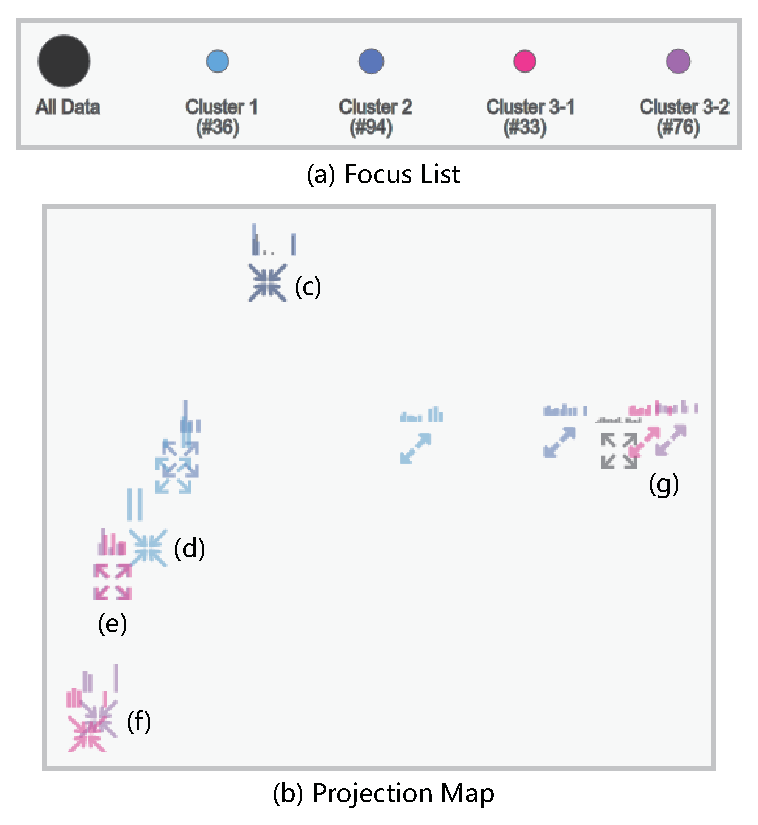
\includegraphics[width=0.85\linewidth]{images/map_1.eps}% 1\linewidth
  \caption{USDA Food Data: we choose a global cluster as the focus, and found outliers }
\label{fig:map}
  \end{figure}

In the above process, we have found outliers and hierarchical clusters in different levels of locality. The four clusters seem layered in the overview(Figure~\ref{fig:food2}(i), (j), Figure~\ref{fig:food3}(g), (h)). Without the featured local projections, it's hard for users to discover and interpret those clusters. Besides, the projections also help to understand the unselected data, and how the focus resembles or differs from them. This will be impossible if the context data are discarded in the projection.

\begin{figure*}[htbp]
\centering
  \includegraphics[width=0.97\linewidth]{images/food_1.eps}% 1\linewidth
  \caption{USDA Food Data: We choose a global cluster as the focus (a), and customize the projection to explore its features (b, c). Outliers can be found in the suggested subspace (d), which are hard to discern in the global projection (f). See Section~\ref{case:food} for more details.}
\label{fig:food1}
  \end{figure*}

\begin{figure*}[htbp]
\centering
  \includegraphics[width=0.97\linewidth]{images/food_2.eps}% 1\linewidth
  \caption{We focus on the cluster found in the subspace (Figure~\ref{fig:food1} (e)). Similarities (b) and diversities (c) are revealed among the cluster members. Three smaller clusters are found. One of them has a strong pattern that it contains no fibers of beta carotene (g). It could be a group of animal-based foods. See Section~\ref{case:food} for more details.}
\label{fig:food2}
  \end{figure*}

\begin{figure*}[htbp]
\centering
  \includegraphics[width=0.97\linewidth]{images/food_3.eps}% 1\linewidth
  \caption{We choose a sub-cluster found in Figure~\ref{food2}(f) to be the new focus. After removing some outliers within the cluster (b), we can see both strong features (d) and interesting inner structures (c) are revealed in the locally enhanced projections. Again, we find two sub-clusters (e, f) within the focus. They seem to be small neighboring clusters in the overview. See Section~\ref{case:food} for more details.}
\label{fig:food3}
  \end{figure*}

\note{compare to histograms: easy to find the most featured dimensions}